{\color{gray}\hrule}
\begin{center}
\section{Methods} \label{sec:methods}
\end{center}
{\color{gray}\hrule}

\begin{multicols}{2}
The goal of this experiment was to investigate how the angular velocity and applied torque influence the precession behavior of the gyroscope. The experimental setup, shown in figure \ref{fig:methods:setup}, consists of a rotating disc mounted on a low-friction axis with two degrees of freedom. To balance the gyroscope, removable counterweights were used. The TISensorTag sensor was mounted on the vertical axis and was used in conjunction with the Phyphox app to measure the angular velocity.
The experiment began with balancing the gyroscope by adjusting the counterweights so no torque was exerted in its free configuration. Once balanced, the rotor disc was manually started. In the first phase of the experiment, the natural behavior of the gyroscope was determined.
In the second phase, torque was applied by placing one or two weights at one end of the rotor axis. The distance between the vertical axis and the center of mass of the weights was measured. The weights were removed and attached at the other end of the rotor axis and the distance was measured again. 
In the third phase, the gyroscope was set in motion, and its behavior was recorded using a digital camera operating at $60$ frames per second to determine the rotor’s time of revolution. These measurements were repeated for the two weight positions to analyze precession behavior under varying torque conditions.
For each part of the experiment, multiple measurements were taken to minimize errors.

\end{multicols}

\begin{figure}[H]
    \centering
    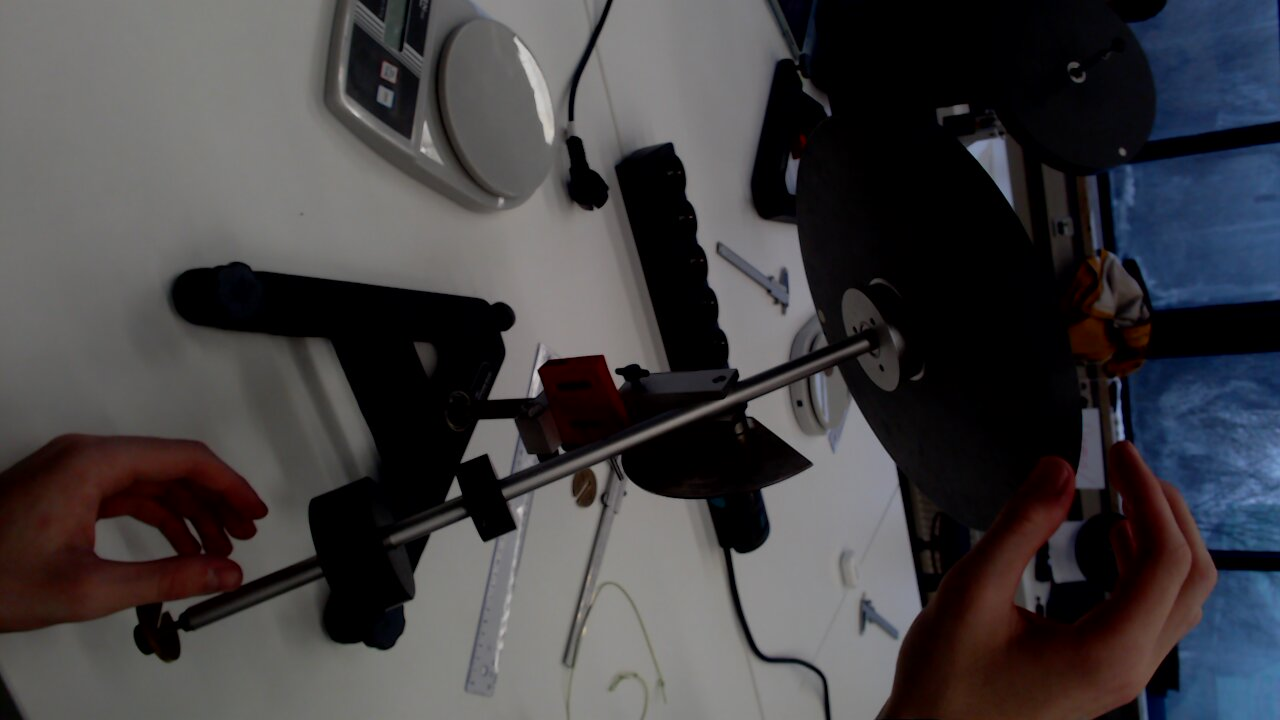
\includegraphics[width=0.5\columnwidth, angle=90]{gyroscope/images/setup}
    \caption{The gyroscope setup.}
    \label{fig:methods:setup}
\end{figure}
